\documentclass[mathserif,11pt]{beamer}

\usepackage{url,verbatim,natbib}
\usepackage[english]{babel}
\usepackage{amsmath, mathabx}
\usepackage{dsfont, ulem}
\usepackage{tikz}
\usepackage{xparse}
\newtheorem{proposition}[theorem]{Proposition}

\usepackage[headheight=22pt]{beamerthemeboxes}
\usepackage{graphicx}
\beamertemplatenavigationsymbolsempty 
\setbeamercovered{transparent}
\usepackage{centernot}

\setbeamertemplate{itemize item}{$\bullet$} 
\setbeamercolor{title}{fg=uio}
\setbeamertemplate{sections/subsections in toc}[ball unnumbered]
\setbeamercolor{section in toc}{fg=uio,bg=white}
\setbeamercolor{subsection in toc}{fg=uio,bg=white}
\setbeamercolor{result}{fg=black, bg=yellow}
\newcommand{\dotsim}{\stackrel{\cdot}{\sim}}
\newcommand{\interi}{{\rm Z}\negthinspace\negthinspace {\rm Z}}
\newcommand{\reali}{{\rm I}\negthinspace {\rm R}}
\newcommand{\naturali}{{\rm I}\negthinspace {\rm N}}
\newcommand{\sign}{\mathop{\rm sgn}\nolimits}
\newcommand{\sgn}{\mathop{\mathrm{sgn}}}
\definecolor{redve}{rgb}{0.604,0.008,0.00}
\definecolor{lmu}{rgb}{0.188,0.522,0.306}
\definecolor{uio}{rgb}{0.847,0.118,0.02}

\def\R{{\rm I\!R}}
\def\P{{\rm Pr}}
\def\Real{{\rm I\!R}}
\def\T{{\footnotesize {^{_{\sf T}}}}}
\def\tr{{\rm tr}}
\def\diag{{\rm diag}}

\NewDocumentCommand\DownArrow{O{2.0ex} O{black}}{%
   \mathrel{\tikz[baseline] \draw [<-, line width=0.5pt, #2] (0,0) -- ++(0,#1);}
}

\useframetitletemplate{% 
\begin{centering} 
\begin{small} \structure{\textcolor{uio} \insertframetitle {\insertframesubtitle}}
\end{small}

\end{centering} 
}

\addheadboxtemplate{\color[rgb]{1,1,1}}{\color{uio} \underline{{\hspace{5pt}\includegraphics[scale=0.06]{../../../../support/uio_logo_eng} \hspace{0.265\paperwidth}\color{black} \tiny  STK-IN4300 - Statistical Learning Methods in Data Science} \hspace{5pt}}}

%\bfseries{\insertsection}

\addfootboxtemplate{\color[rgb]{1,1,1}}{\color{black} \tiny \quad  
STK-IN4300: lecture 6
  \hfill \tiny \insertframenumber / \inserttotalframenumber \hspace{5pt}}

  
\title{STK-IN4300 \\ Statistical Learning Methods in Data Science}
\author{Riccardo De Bin} 
\institute{debin@math.uio.no} 
\date{}


\begin{document}
\setbeamercolor{bgr}{fg=black,bg=uio}

{
\setbeamertemplate{headline}{}
\frame{
\vspace{-2cm}
\begin{beamercolorbox}[sep=-2.2em,wd=5cm,colsep=0.5pt,ht=4.25ex,dp=3ex,left]{postit}
\includegraphics[scale=0.06]{../../../../support/uio_logo_eng}
\end{beamercolorbox}
\vspace{0.365cm}
\noindent\makebox[\linewidth]{\color{uio} \rule{\paperwidth}{0.4pt}}
\vspace{2.5cm}
\titlepage
}
}

\frame{\frametitle{Outline of the lecture}
\tableofcontents
}


\section{Kernel Smoothing Methods}

\subsection{One dimensional kernel smoothers}

\frame{\frametitle{One dimensional kernel smoothers: }
\framesubtitle{from $k$NN to kernel smoothers}
\begin{columns}
\begin{column}{0.5\textwidth}
When we introduced the \textcolor{uio}{$k$NN} algorithm,
$$
\hat{f}(x) = \text{Ave}(y_i|x_i\in N_k(x))
$$
\vspace{-15pt}
\begin{itemize}
\item justified as an estimate of $E[Y|X=x]$.
\item[]
\end{itemize}

Drawbacks:
\begin{itemize}
\item ugly \textcolor{uio}{discontinuities};
\item \textcolor{uio}{same weight} to all points despite their distance to $x$.
\end{itemize}
\end{column}
\begin{column}{0.5\textwidth}
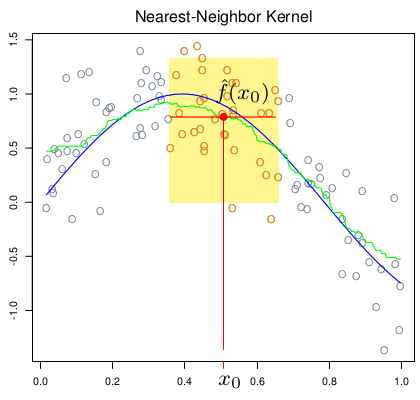
\includegraphics[width=\textwidth]{figure6_1_left}
\end{column}
\end{columns}
}


\frame{\frametitle{One dimensional kernel smoothers: }
\framesubtitle{definition}
Alternative: weight the effect of each point based on its \textcolor{uio}{distance}.
$$
\hat{f}(x_0) = \frac{\sum_{i=1}^N K(x_0,x_i)y_i}{\sum_{i=1}^N K(x_0,x_i)},
$$
where
\begin{equation}\label{kernel}
K_\lambda(x_0,x) = D\left(\frac{|x-x_0|}{\lambda}\right).
\end{equation}
Here:
\begin{itemize}
\item $D(\cdot)$ is called \textcolor{uio}{kernel};
\item $\lambda$ is the bandwidth or \textcolor{uio}{smoothing parameter}.
\end{itemize}
}


\frame{\frametitle{One dimensional kernel smoothers: }
\framesubtitle{comparison}
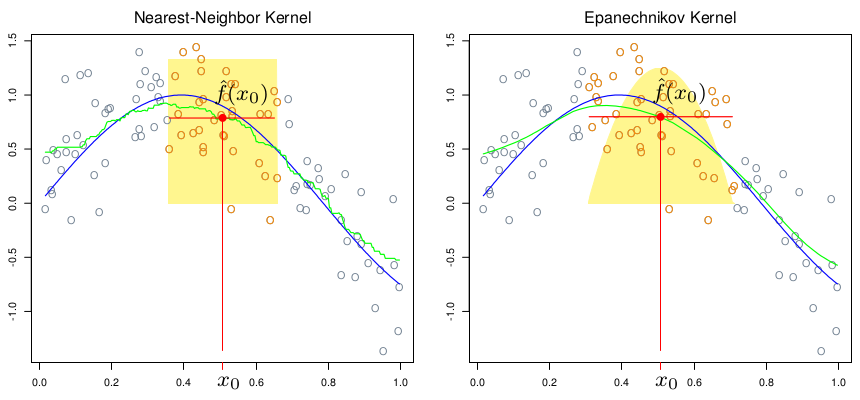
\includegraphics[width=\textwidth]{figure6_1}
}


\frame{\frametitle{One dimensional kernel smoothers: }
\framesubtitle{typical kernels}
We need to choose \textcolor{uio}{$D(\cdot)$}:
\begin{itemize}
\item \textcolor{uio}{symmetric} around $x_0$;
\item goes off \textcolor{uio}{smoothly} with the distance.
\item[]
\end{itemize}
Typical choices:
\begin{center}
\renewcommand{\arraystretch}{1.5}
\begin{tabular}{lcc}
Nucleus & D(t) & Support \\
\hline
Normal & $\frac{1}{\sqrt{2\pi}}\exp\{-\frac{1}{2}t^2\}$ & $\mathds{R}$\\
Rectangular & $\frac{1}{2}$ & $(-1,1)$\\
Epanechnikov & $\frac{3}{4}(1-t^2)$ & $(-1,1)$\\
Biquadratic & $\frac{15}{16}(1-t^2)^2$ & $(-1,1)$\\
Tricubic & $\frac{70}{81}(1-|t|^3)^3$ & $(-1,1)$ \\
\hline
\end{tabular}
\end{center}
}


\frame{\frametitle{One dimensional kernel smoothers: }
\framesubtitle{comparison}
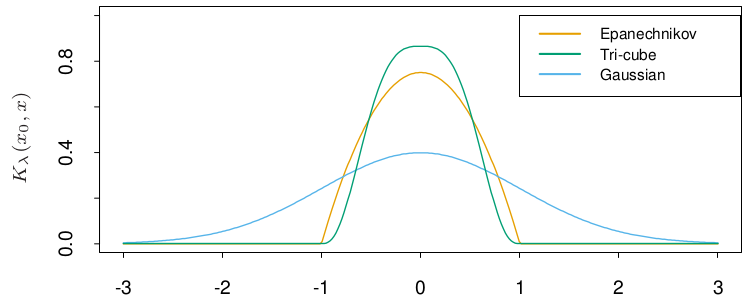
\includegraphics[width=\textwidth]{figure6_2}
}



\frame{\frametitle{One dimensional kernel smoothers: }
\framesubtitle{choice of the smoothing parameter}
Choice of the \textcolor{uio}{bandwidth $\lambda$}:
\begin{itemize}
\item controls \textcolor{uio}{how large} is the interval around $x_0$ to consider,
\begin{itemize}
\item for Epanechnikov, biquadratic or tricubic kernels $\rightarrow$ \textcolor{uio}{radius} of the support;
\item for Gaussian kernel, \textcolor{uio}{standard deviation};
\end{itemize}
\item \textcolor{uio}{large values} implies lower variance but higher \textcolor{uio}{bias},
\begin{itemize}
\item $\lambda$ \textcolor{uio}{small} $\rightarrow$ $\hat{f}(x_0)$ based on few points $\rightarrow$ $y_i$'s \textcolor{uio}{closer} to $y_0$;
\item $\lambda$ \textcolor{uio}{large} $\rightarrow$ more points $\rightarrow$ \textcolor{uio}{stronger} effect of averaging;
\end{itemize}
\item alternatively,
\begin{itemize}
\item \textcolor{uio}{adapt} to the local density (fix $k$ as in $k$NN);
\item expressed by substituting $\lambda$ with \textcolor{uio}{$h_\lambda(x_0)$} in \eqref{kernel};
\item keep bias \textcolor{uio}{constant}, variance is \textcolor{uio}{inversely proportional} to the local density.
\end{itemize}
\end{itemize}
}


\frame{\frametitle{One dimensional kernel smoothers: }
\framesubtitle{effect of the smoothing parameter}
\centering
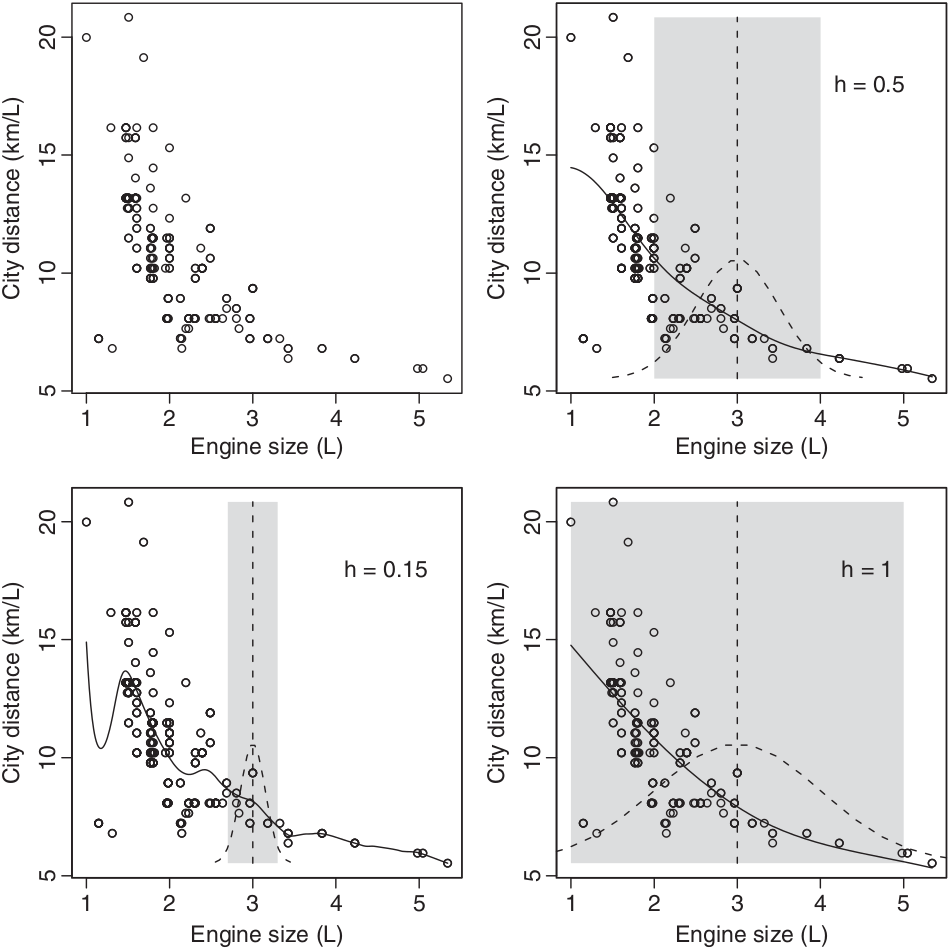
\includegraphics[width=0.7\textwidth]{band}
}


\subsection{Selecting the width of a kernel}

\frame{\frametitle{Selecting the width of a kernel: }
\framesubtitle{bias and variance}
Assume $y_i = f(x_i) + \epsilon_i$, $\epsilon_i$ i.i.d.\ s.t.\ $E[\epsilon_i] = 0$ and $\text{Var} = \sigma^2$, then
$$
E[\hat{f}(x)] \approx f(x) + \frac{\lambda^2}{2}\sigma_D^2f''(x)
$$
and
$$
\text{Var}[\hat{f}(x)] \approx \frac{\sigma^2}{N\lambda}\frac{R_D}{g(x)}
$$
for $N$ large and $\lambda$ sufficiently close to 0 \citep{AzzaliniScarpa2012}.

Here:
\begin{itemize}
\item $\sigma_D^2 = \int t^2 D(t) dt$;
\item $R_D = \int D(t)^2 dt$;
\item $g(x)$ is the density from which the $x_i$ were sampled.
\end{itemize}
}


\frame{\frametitle{Selecting the width of a kernel: }
\framesubtitle{bias and variance}
Note:
\begin{itemize}
\item the \textcolor{uio}{bias} is a multiple of \textcolor{uio}{$\lambda^2$};
\begin{itemize}
\item $\lambda\rightarrow 0$ reduce the bias;
\end{itemize}
\item the \textcolor{uio}{variance} is a multiple of \textcolor{uio}{$\frac{1}{N\lambda}$};
\begin{itemize}
\item $\lambda\rightarrow \infty$ reduce the variance.
\end{itemize}
\item[]
\end{itemize}

The quantities $g(x)$ and $f''(x)$ are unknown, otherwise
$$
\lambda_\text{opt} =\left(\frac{\sigma^2R_D}{\sigma^4_Df''(x)g(x)N}\right)^{1/5};
$$
note that $\lambda$ must tend to 0 with rate $N^{-1/5}$ (i.e., \textcolor{uio}{very slowly}).
}


\frame{\frametitle{Selecting the width of a kernel: }
\framesubtitle{AIC}
Anyway, local smoothers are \textcolor{uio}{linear estimators},
$$
\hat{f}(x) = S_\lambda y
$$
as $S_\lambda$, the smoothing matrix, does \textcolor{uio}{not depend} on $y$.

\vspace{12pt}

Therefore, an \textcolor{uio}{Akaike Information Criterion} can be implemented,
$$
AIC = \log \hat{\sigma} + 2\;\text{trace}\{S_\lambda\}
$$
where $\text{trace}\{S_\lambda\}$ are the \textcolor{uio}{effective degrees of freedom}.

\vspace{12pt}

Otherwise it is always possible to implement a \textcolor{uio}{cross-validation} procedure.
}


\frame{\frametitle{One dimensional Kernel Smoothers: }
\framesubtitle{other issues}
Other points to consider:
\begin{itemize}
\item \textcolor{uio}{boundary issues}:
\begin{itemize}
\item estimates are \textcolor{uio}{less accurate} close to the boundaries;
\item less observations;
\item \textcolor{uio}{asymmetry} in the kernel;
\end{itemize}
\item \textcolor{uio}{ties} in the $x_i$'s:
\begin{itemize}
\item possibly more weight on a single $x_i$;
\item there can be different $y_i$ for the same $x_i$.
\end{itemize}
\end{itemize}
}


\subsection{Local linear regression}

\frame{\frametitle{Local linear regression: }
\framesubtitle{problems at the boundaries}
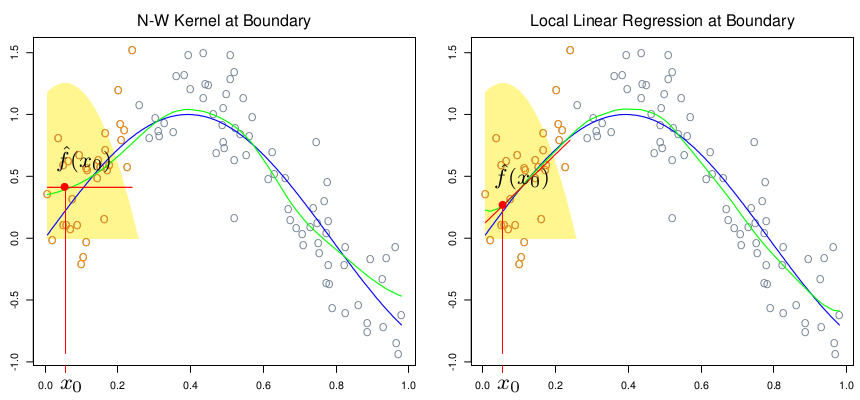
\includegraphics[width=\textwidth]{figure6_3}
}


\frame{\frametitle{Local linear regression: }
\framesubtitle{problems at the boundaries}
By fitting a \textcolor{uio}{straight line}, we solve the problem to the first order.
\vspace{-12pt}
$$
\downarrow
$$
\vspace{-36pt}
\begin{center}
{\bf Local linear regression}
\end{center}

Locally weighted linear regression solve, at each target point $x_0$,
$$
\min_{\alpha(x_0), \beta(x_0)} \sum_{i=1}^N K_\lambda(x_0,x_i)[y_i - \alpha(x_0) - \beta(x_0)x_i]^2.
$$
The estimate is $\hat{f}(x_0) = \hat{\alpha}(x_0) + \hat{\beta}(x_0)x_0$:
\begin{itemize}
\item the model is fit on all data belonging to the \textcolor{uio}{support} of $K_\lambda$;
\item it is \textcolor{uio}{only} evaluated in $x_0$.
\end{itemize}
}


\frame{\frametitle{Local linear regression: }
\framesubtitle{estimation}
Estimation
\begin{align*}
\hat{f}(x_0) &= b(x_0)^T(B^TW(x_0)B)^{-1}B^TW(x_0)y\\
&= \sum_{i=1}^N l_i(x_0)y_i,
\end{align*}
where:
\begin{itemize}
\item $b(x_0)^T = (1,x_0)$
\item $B = (\vec{1},X)$;
\item $W(x_0)$ is a $N\times N$ diagonal matrix with $i$-th term $K_\lambda(x_0,x_i)$;
\item $\hat{f}(x_0)$ is \textcolor{uio}{linear} in $y$ ($l_i(x_0)$ does not depend on $y_i$);
\item the weights $l_i(x_0)$ are sometimes called \textcolor{uio}{equivalent kernels},
\begin{itemize}
\item \textcolor{uio}{combine} the weighting kernel $K_\lambda(x_0,\cdot)$ and the LS operator.
\end{itemize}
\end{itemize}
}


\frame{\frametitle{Local linear regression: }
\framesubtitle{bias correction due asymmetry}
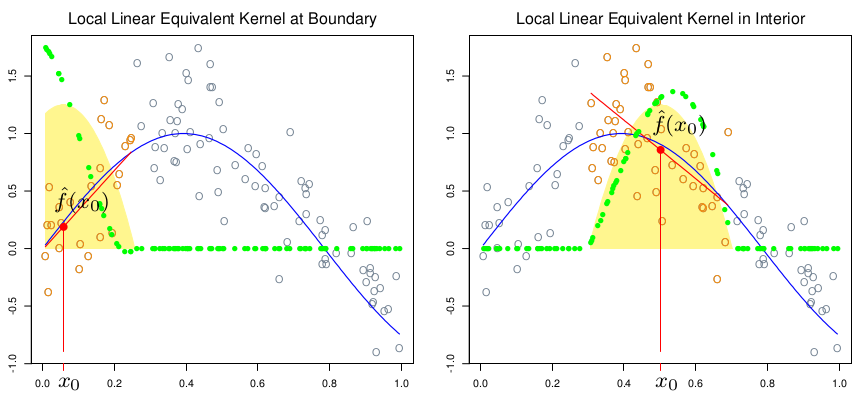
\includegraphics[width=\textwidth]{figure6_4}
}


\frame{\frametitle{Local linear regression: }
\framesubtitle{bias}
Using a Taylor expansion of $f(x_i)$ around $x_0$,
\begin{align}\label{taylor}
E[\hat{f}(x_0)] =& \sum_{i=1}^N l_i(x_0)f(x_i)\nonumber\\
=& f(x_0)\sum_{i=1}^N l_i(x_0) + f'(x_0)\sum_{i=1}^N (x_i - x_0) l_i(x_0) +\nonumber\\
 &+\frac{f''(x_0)}{2}\sum_{i=1}^N (x_i - x_0)^2 l_i(x_0) + \dots
\end{align}
For local linear regression,
\begin{itemize}
\item $\sum_{i=1} l_i(x_0) = 1$;
\item $\sum_{i=1}^N (x_i - x_0) l_i(x_0) = 0$.
\end{itemize}
Therefore,
\begin{itemize}
\item $E[\hat{f}(x_0)] - f(x_0) = \frac{f''(x_0)}{2}\sum_{i=1}^N (x_i - x_0)^2 l_i(x_0) + \dots$.
\end{itemize}
}


\subsection{Local polynomial regression}

\frame{\frametitle{Local polynomial regression: }
\framesubtitle{bias}
Why \textcolor{uio}{limiting} to a linear fit?
$$
\min_{\alpha(x_0), \beta_1(x_0),\dots,\beta_d(x_0)} \sum_{i=1}^N K_\lambda(x_0,x_i)\left[y_i - \alpha(x_0) - \sum_{j=1}^d \beta_j(x_0)x_i^j\right]^2,
$$
with solution $\hat{f(x_0)} = \hat{\alpha}(x_0) + \sum_{j=1}^d\hat{\beta}(x_0)x_0^j$.

\vspace{12pt}
\begin{itemize}
\item it can be shown that the bias, using \eqref{taylor}, \textcolor{uio}{only} involves components of \textcolor{uio}{degree $d+1$};
\item in contrast to local linear regression, it tends to be \textcolor{uio}{closer} to the true function in regions with \textcolor{uio}{high curvature},
\begin{itemize}
\item \textcolor{uio}{no} {\it trimming the hills and filling the gaps} effect.
\end{itemize}
\end{itemize}
}


\frame{\frametitle{Local polynomial regression: }
\framesubtitle{regions with high curvature}
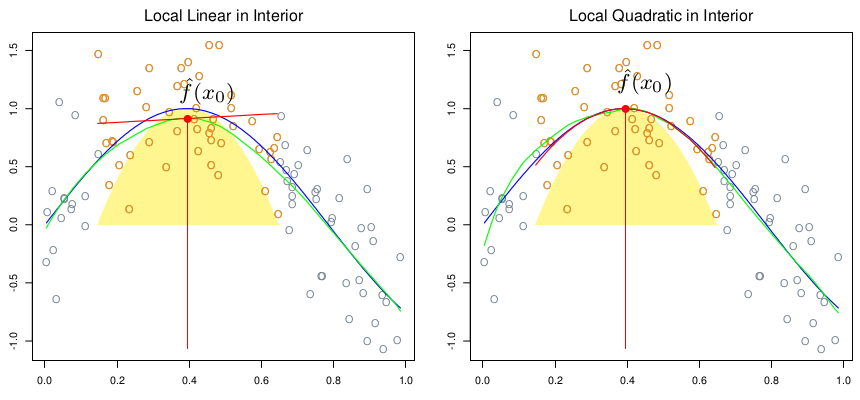
\includegraphics[width=\textwidth]{figure6_5}
}


\frame{\frametitle{Local polynomial regression: }
\framesubtitle{bias-variance trade-off}
Not surprisingly, there is a \textcolor{uio}{price} for having less bias.

\vspace{12pt}

Assuming a model $y_i = f(x_i) + \epsilon_i$, where $\epsilon_i$ are i.i.d.\ with mean $0$ and variance $\sigma^2$,
$$
\text{Var}(\hat{f}(x_i)) = \sigma^2||l(x_0)||
$$
It can be shown that \textcolor{uio}{$||l(x_0)||$ increase with $d$} $\Rightarrow$ bias-variance trade-off in the choice of $d$.
}


\frame{\frametitle{Local polynomial regression: }
\framesubtitle{variance}
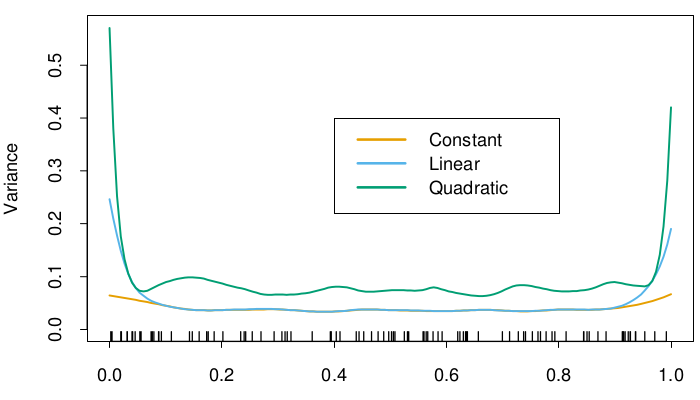
\includegraphics[width=\textwidth]{figure6_6}
}


\frame{\frametitle{Local polynomial regression: }
\framesubtitle{final remarks}
Some final remarks:
\begin{itemize}
\item local linear fits \textcolor{uio}{help dramatically} in alleviating boundary issues;
\item quadratic fits do a \textcolor{uio}{little better}, but \textcolor{uio}{increase variance};
\item quadratic fits solve issues in \textcolor{uio}{high curvature} regions;
\item asymptotic analyses suggest that polynomials of odd degrees \textcolor{uio}{should be preferred} to those of even degrees,
\begin{itemize}
\item the MSE is \textcolor{uio}{asymptotically dominated} by boundary effects;
\end{itemize}
\item anyway, the choice of $d$ is \textcolor{uio}{problem specific}.
\end{itemize}
}


\subsection{Local regression in $\mathds{R}^p$}

\frame{\frametitle{Local regression in $\mathds{R}^p$: }
\framesubtitle{extension}
Kernel smoothing and local regression can be easily generalized to \textcolor{uio}{more dimensions}:
\begin{itemize}
\item average weighted by a kernel with \textcolor{uio}{support in $\mathds{R}^p$};
\item for local regression, fit locally an \textcolor{uio}{hyperplane}.
\end{itemize}
\vspace{6pt}
\begin{columns}
\begin{column}{0.4\textwidth}
With \textcolor{uio}{$d=1$} and \textcolor{uio}{$p=2$},
\begin{itemize}
\item $b(X) = (1,X_1,X_2)$
\end{itemize}
\end{column}
\begin{column}{0.6\textwidth}
With \textcolor{uio}{$d=2$} and \textcolor{uio}{$p=2$},
\begin{itemize}
\item $b(X) = (1,X_1,X_2,X_1^2,X_2^2,X_1X_2)$
\end{itemize}
\end{column}
\end{columns}
At each $x_0$, solve
$$
\min_{\beta(x_0)} \sum_{i=1}^N K_\lambda(x_0,x_i)[y_i - b(x_i)^T\beta(x_0)x_i]^2.
$$
where $K_\lambda(x_0,x_i)$ is a \textcolor{uio}{radial function},
$$
K_\lambda(x_0,x_i) = D\left(\frac{||x-x_0||}{\lambda}\right).
$$
Since $||\cdot||$ is the Euclidean norm, \textcolor{uio}{standardize} each $x_j$.
}


\frame{\frametitle{Local regression in $\mathds{R}^p$: }
\framesubtitle{example}
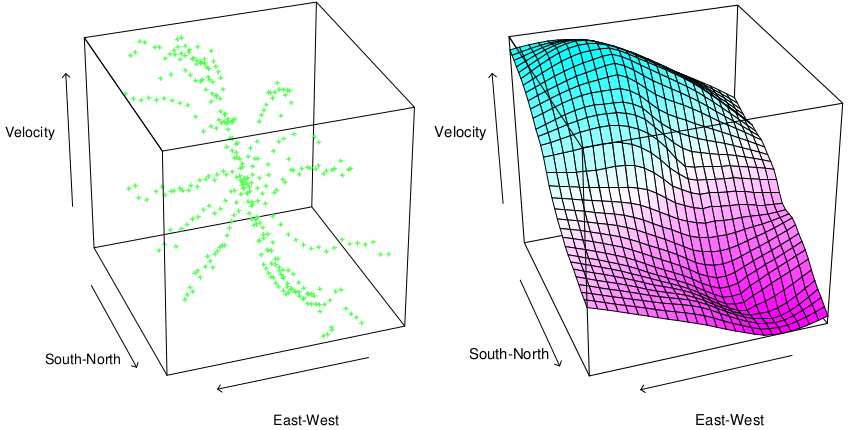
\includegraphics[width=\textwidth]{figure6_8}
}

\frame{\frametitle{Local regression in $\mathds{R}^p$: }
\framesubtitle{remarks}
Some remarks:
\begin{itemize}
\item boundary issues are even \textcolor{uio}{more dramatic} than in one dimension;
\begin{itemize}
\item the fraction of points at the boundary \textcolor{uio}{increases} to 1 by \textcolor{uio}{increasing} the dimensions;
\item \textcolor{uio}{curse of dimensionality};
\end{itemize}
\item local polynomials \textcolor{uio}{still} perform boundary corrections up to the desired order;
\item local regression \textcolor{uio}{does not} make really sense for $d>3$,
\begin{itemize}
\item it is \textcolor{uio}{impossible} to maintain \textcolor{uio}{localness} (small bias) and \textcolor{uio}{sizeable sample} in the neighbourhood (small variance);
\item again, \textcolor{uio}{curse of dimensionality}.
\end{itemize}
\end{itemize}
}


\subsection{Structured local regression models in $\mathds{R}^p$}

\frame{\frametitle{Structured local regression models in $\mathds{R}^p$: }
\framesubtitle{structured kernels}
When the ratio sampe size/dimensions is \textcolor{uio}{too large}:

\vspace{12pt}

{\bf \uline{Structured kernels}}
$$
K_{\lambda,A}(x_0,x)=D\left(\frac{(x-x_0)^TA(x-x_0)}{\lambda}\right)
$$
\begin{itemize}
\item $A$ is a matrix semidefinite positive;
\item we can \textcolor{uio}{add structures} through $A$:
\begin{itemize}
\item $A$ diagonal, increase or decrease the \textcolor{uio}{importance of the predictor} $X_j$ by increasing/decreasing $a_{jj}$;
\item \textcolor{uio}{low rank} versions of $A$ $\rightarrow$ projection pursuit;
\end{itemize}
\end{itemize}
}


\frame{\frametitle{Structured local regression models in $\mathds{R}^p$: }
\framesubtitle{structured regression functions}
{\bf \uline{Structured regression functions}}
$$
f(X_1,\dots,X_p) = \alpha + \sum_{j=1}^p g_j(X_j) + \sum_{k<\ell}g_{k\ell}(X_k, X_\ell) + \dots
$$
\begin{itemize}
\item we can \textcolor{uio}{simplify} the structure;
\item examples:
\begin{itemize}
\item remove all \textcolor{uio}{interaction terms},\\
$f(X_1,\dots,X_p) = \alpha + \sum_{j=1}^p g_j(X_j)$;
\vspace{6pt}
\item keep only the \textcolor{uio}{first order} interactions,\\
$f(X_1,\dots,X_p) = \alpha + \sum_{j=1}^p g_j(X_j) + \sum_{k<\ell}g_{k\ell}(X_k, X_\ell)$;
\vspace{6pt}
\item \dots
\end{itemize}
\end{itemize}
}


\frame{\frametitle{Structured local regression models in $\mathds{R}^p$: }
\framesubtitle{varying coefficient models}
{\bf \uline{Varying coefficient models}}

\vspace{12pt}
The \textcolor{uio}{varying coefficient models}:
\begin{itemize}
\item are a \textcolor{uio}{special case} of structured regression functions;
\item consider \textcolor{uio}{only $q<p$} predictors, all the remaining are in $Z$;
\item assume the \textcolor{uio}{conditionally} linear model,
$$
f(X)=\alpha(Z) + \beta_1(Z)X_1 + \dots + \beta_q(Z)X_q;
$$
\item \textcolor{uio}{given $Z$}, it is a linear model,
\begin{itemize}
\item solution via least squares estimator;
\end{itemize}
\item the coefficients \textcolor{uio}{can vary} with $Z$.
\end{itemize}
}


\frame{\frametitle{Structured local regression models in $\mathds{R}^p$: }
\framesubtitle{structured regression functions}
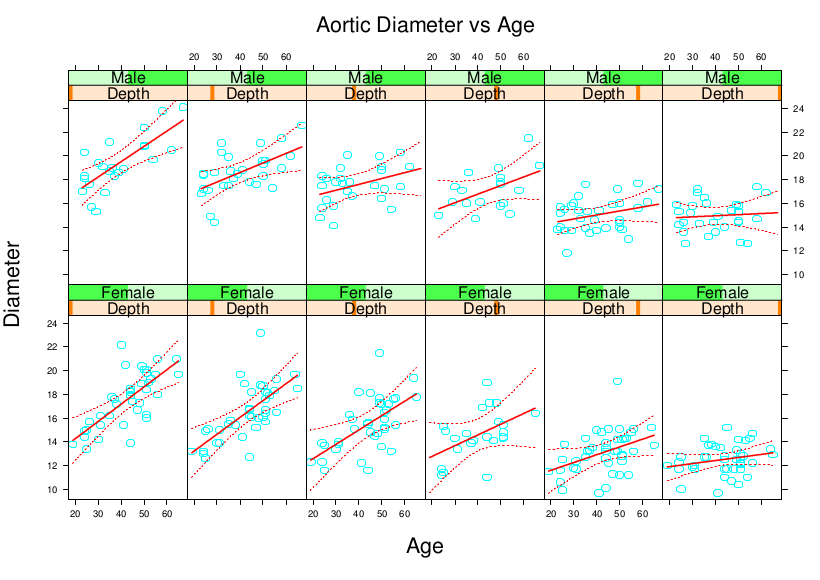
\includegraphics[width=\textwidth]{figure6_10}
}


\subsection{Kernel density estimation}

\frame{\frametitle{Kernel density estimation: }
\framesubtitle{density estimation}
Suppose to have a random sample, $x_i \in \mathds{R}$, $i=1,\dots, N$, and want to \textcolor{uio}{estimate its density $f_X(x)$}. An estimation at each point $x_0$ is
$$
\hat{f}_X(x_0) = \frac{\#x_i \in \mathcal{N}(x_0)}{N\lambda}.
$$
where $\mathcal{N}(x_0)$ is a small \textcolor{uio}{metric neighborhood} around $x_0$ of width $\lambda$.

\vspace{12pt}

Bumpy estimate $\rightarrow$ the {\bf smooth Parzen estimate} is \textcolor{uio}{preferred},
$$
\hat{f}_X(x_0) = \frac{1}{N\lambda} \sum_{i=1}^N K_\lambda(x_0,x_i),
$$
in which closer observations contributes \textcolor{uio}{more}.
}


\frame{\frametitle{Kernel density estimation: }
\framesubtitle{choice of $K_\lambda(x_0,x)$}
For the smooth Parzen estimate, the \textcolor{uio}{Gaussian kernel} is often used,
$$
K_\lambda(x_0,x) = \phi\left(\frac{|x - x_0|}{\lambda}\right)
$$
where $\phi$ is the density of a standard normal.

\vspace{12pt}

Using the density of a normal with mean 0 and sd $\lambda$, denoted $\phi_\lambda$,
\begin{align*}
{f}_X(x) &= \frac{1}{N} \sum_{i=1}^N \phi_\lambda(x - x_i)\\
&= (\hat{F} \star \phi_\lambda)(x)
\end{align*}
the \textcolor{uio}{convolution} of the sample empirical distribution \textcolor{uio}{$\hat{F}$} with \textcolor{uio}{$\phi_\lambda$}:
\begin{itemize}
\item smooth $\hat{F}$ by \textcolor{uio}{adding independent Gaussian noise} to each $x_i$.
\end{itemize}
}


\frame{\frametitle{Kernel density estimation: }
\framesubtitle{example}
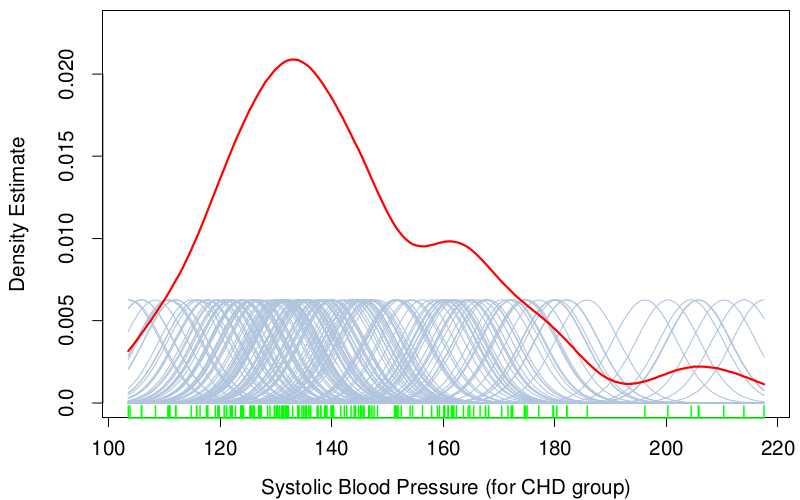
\includegraphics[width=\textwidth]{figure6_13}
}


\subsection{Mixture models for density estimation}

\frame{\frametitle{Mixture models for density estimation: }
\framesubtitle{density estimation}
The density $f(X)$ can be considered a \textcolor{uio}{mixture} of distributions,
$$
f(X)= \sum_{m=1}^M \alpha_m g(x;\mu_m, \Sigma_m)
$$
where
\begin{itemize}
\item $\alpha_M$ are the \textcolor{uio}{mixing proportions}, $\sum_{m=1}^M \alpha_M = 1$;
\item each \textcolor{uio}{density $g(\cdot)$} has mean $\mu_m$ ad covariance $\Sigma_m$;
\item almost always \textcolor{uio}{$g(x;\mu_m, \Sigma_m) = \phi(g(x;\mu_m, \Sigma_m))$};
\item[] \hspace{60pt} $\downarrow$
\item {\bf Gaussian mixture model}.
\end{itemize}
}


\frame{\frametitle{Mixture models for density estimation: }
\framesubtitle{example}
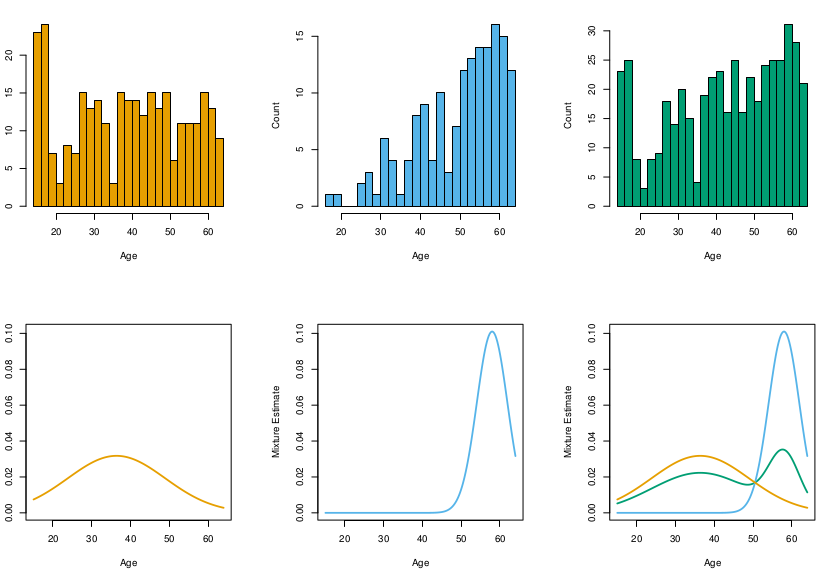
\includegraphics[width=\textwidth]{figure6_17}
}



\section{Nonparametric Density Estimation with a Parametric Start}

\frame{\frametitle{Semiparametric density estimation: }
\framesubtitle{\cite{HjortGlad1995}}
\textcolor{uio}{\cite{HjortGlad1995}} proposed a different option:
\begin{itemize}
\item \textcolor{uio}{start} with a \textcolor{uio}{parametric} density estimate $f_0(x,\hat{\theta})$;
\item multiply it to a \textcolor{uio}{correction term} $r(x)=f(x)/f_0(x,\hat{\theta})$;
\item estimate the correction term with a \textcolor{uio}{kernel smoother},
$$
\hat{r}(x) = \frac{1}{N}\sum_{i=1}^N \frac{K_\lambda(x,x_i)}{f_0(x_i,\hat{\theta})};
$$
\item the resulting \textcolor{uio}{density estimate} is
$$
\hat{f}_{HG}(x) = f_0(x,\hat{\theta}) \hat{r}(x) = \frac{1}{N}\sum_{i=1}^N K_\lambda(x,x_i)\frac{f_0(x,\hat{\theta})}{f_0(x_i,\hat{\theta})}.
$$
\end{itemize}
}


\frame{\frametitle{Semiparametric density estimation: }
\framesubtitle{\cite{HjortGlad1995}}
Note that:
\begin{itemize}
\item the initial parametric estimate is \textcolor{uio}{not necessarily} a good approximation to the true density:
\begin{itemize}
\item the method often works well with \textcolor{uio}{``bad'' parametric starts};
\item the \textcolor{uio}{better} the approximation, the \textcolor{uio}{better} the result, though;
\end{itemize}
\item $f_0(x,\hat{\theta}) = \text{constant} \rightarrow \textcolor{uio}{f_0(x) \sim \text{Unif}}$,
\begin{itemize}
 \item back to the \textcolor{uio}{classic kernel estimator}.
\end{itemize}
\end{itemize}
}


\frame{\frametitle{Semiparametric density estimation: }
\framesubtitle{properties}
Consider $f_{HG}(x)$'s \textcolor{uio}{variance},
$$
\text{Var}(\hat{f}_{HG}(x)) = \text{Var}(\hat{f}_\text{kernel}(x)) + O\left(\frac{\lambda}{N} + \frac{1}{N^2}\right),
$$
\vspace{-12pt}
\begin{itemize}
\item $\hat{f}_{HG}(x)$ and $\hat{f}_\text{kernel}(x)$ have \textcolor{uio}{approximatively the same} variance;
\item[]
\end{itemize}
and \textcolor{uio}{bias},
$$
E[\hat{f}_{HG}(x)] \approx f(x) + \frac{\lambda^2}{2}\sigma_D^2f_0(x)r''(x),
$$
\vspace{-12pt}
\begin{itemize}
\item \textcolor{uio}{same order} as the bias of $\hat{f}_\text{kernel}(x)$, i.e., \textcolor{uio}{O($\lambda^2$)};
\item it is proportional to \textcolor{uio}{$f_0(x)r''(x)$} rather than $f''(x)$;
\item smaller when $f''(x) = f_0''(x)r(x) + 2 f_0'(x)r'(x) + f_0(x)r''(x)$,
\begin{itemize}
\item when $f_0(x)$ is a \textcolor{uio}{good guess}, better performance!
\end{itemize}
\end{itemize}
}


\frame{\frametitle{Semiparametric density estimation: }
\framesubtitle{derivation example}
Example with a \textcolor{uio}{Gaussian start},
\begin{align*}
\hat{f}_{HG}(x) &= f_0(x,\hat{\theta}) \hat{r}(x) = \frac{1}{N}\sum_{i=1}^N K_\lambda(x,x_i)\frac{f_0(x,\hat{\theta})}{f_0(x_i,\hat{\theta})}\\
&= \frac{1}{\hat{\sigma}}\phi\left(\frac{x-\hat{\mu}}{\hat{\sigma}}\right)\frac{\frac{1}{N}\sum_{i=1}^N K_\lambda(x,x_i)}{\phi\left(\frac{x_i-\hat{\mu}}{\hat{\sigma}}\right)}\\
&=\frac{1}{N}\sum_{i=1}^N K_\lambda(x,x_i)\frac{\exp\left\{-\frac{1}{2}\frac{x-\hat{\mu}}{\hat{\sigma}}\right\}}{\exp\left\{-\frac{1}{2}\frac{x-\hat{\mu}}{\hat{\sigma}}\right\}}.
\end{align*}
}


\frame{\frametitle{Semiparametric density estimation: }
\framesubtitle{data example}
\centering
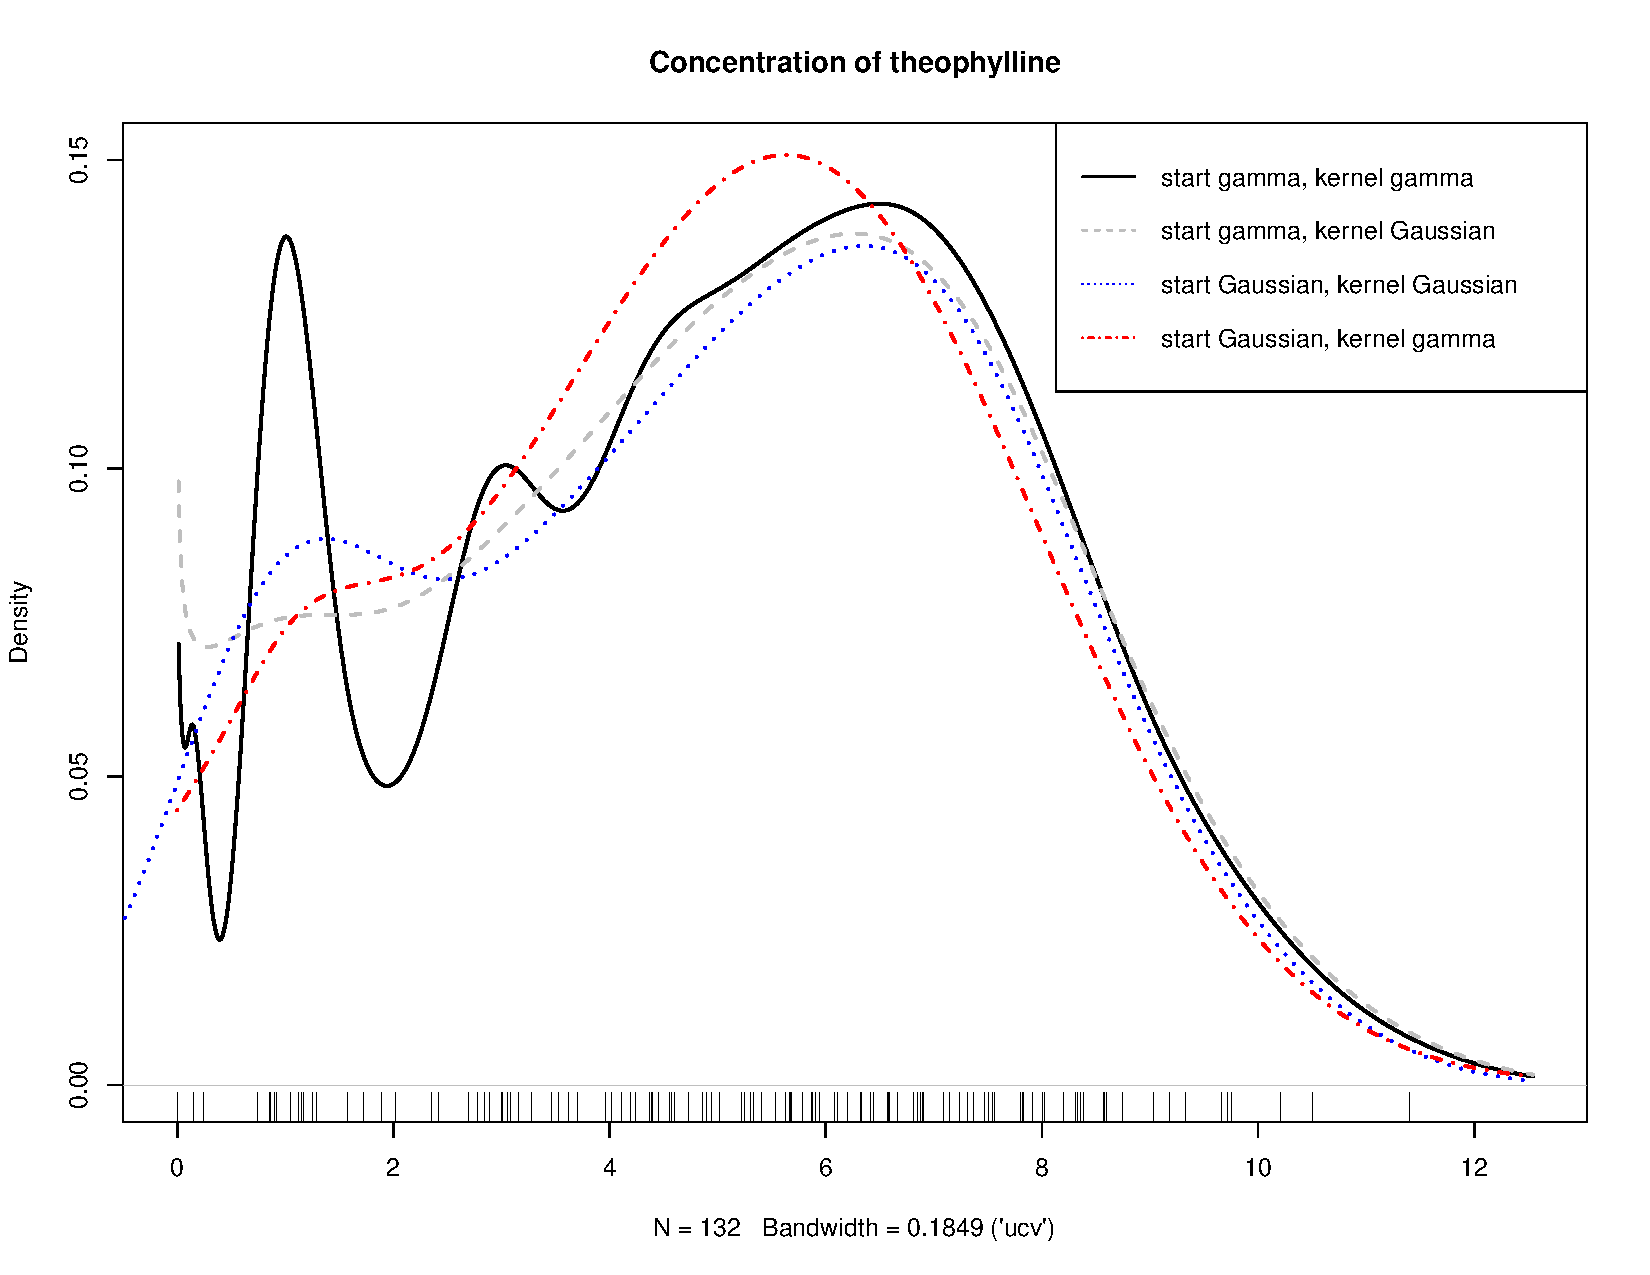
\includegraphics[width=0.92\textwidth]{plotHG}
}



%%%%%%%%%%%
\section*{Bibliography}
%%%%%%%%%%%

\frame[allowframebreaks]{\frametitle{References}
\footnotesize
\bibliographystyle{../../../../support/biometrika}
\bibliography{../../../../support/biblio}
}

\end{document}
